\section{Simulation}
Pour nous permettre d'expérimenter ces architectures nous allons adopter une approche par simulation. La simulation présente de nombreux avantages, notamment le fait de pouvoir accélérer le temps. La simulation étant déterministe, on peut par ailleurs rejouer des scénarios qu'il serait impossible de rejouer par expérimentations sur plateformes réelles (perturbations dans le réseau, par exemple latence). De plus, la simulation peut s'exécuter sur des machines moins puissantes que celles simulées. Enfin, la simulation est automatisable et permet d'éviter d'avoir à réunir des personnes réelles jouant au jeu pour tester les algorithmes qui seront implémentés dans le système contrairement à de l'expérimentation.\\

Comme la simulation est compliquée à réaliser, nous allons nous baser sur un c\oe{}ur de simulation déjà existant et développer notre solution par dessus. Nous n'aurons donc pas à simuler le temps qui s'écoule, le réseau et le CPU dans la simulation mais juste à développer un outil permettant de tester des algorithmes et de mesurer leur efficacité en utilisant les métriques citées plus haut. Pour permettre au simulateur d'être utilisé pour une grande variété de jeux, il sera également nécessaire de fournir une couche d'abstraction sur laquelle le simulateur se basera.

\subsection{Comparaison des simulateurs}
De nombreux simulateurs existent mais utilisent différents niveaux d'approximation. Une simulation trop fidèle demanderait beaucoup de ressources et s'exécuterait très lentement. Inversement, une simulation trop peu fidèle entraînerait des incohérences au niveau des résultats et certains effets de bord ne seraient plus visible (congestion TCP, effet de trafics croisés...). Trouver un bon compromis est donc important pour effectuer notre simulation.\\

Comme la réduction de l'encombrement réseau est important dans notre architecture, il faut que le réseau soit simulé de façon correcte et sans trop d'approximations. Un simulateur tel que PeerSim~\cite{peersim} n'est donc pas envisageable car il n'y a aucune gestion du débit des connexions. En effet, dans ce type de simulateur, un client peut recevoir plus de paquets que sa connexion ne pourrait le supporter par exemple.\\

Une autre partie importante du simulateur est la capacité à gérer les architectures de type cloud, c'est à dire gérer un nombre de serveur dynamique (et théoriquement infini) de machines virtuelles. Dans certains clouds, la puissance des VMs peuvent également varier au cours du temps, les VMs pouvant être relocalisées ou redimensionnées pendant l'exécution. La liste de simulateurs présentée n'est pas exhaustive mais correspond aux plus utilisés et documentés dans le domaine de la recherche.

\paragraph{CloudSim\\}
CloudSim~\cite{cloudsim} est un ensemble d'outils non graphiques servant à la simulation de cloud. CloudSim permet d'avoir des résultats sur la simulation de cloud sans avoir à se soucier des détails d'implémentation bas niveau. Tout les composants simulés de CloudSim communiquent entre eux en utilisant des messages. CloudSim permet également de simuler l'allocation des machines virtuelles, la consommation électrique et le comportement du réseau. CloudSim sert principalement à simuler une infrastructure de cloud et non une application s'exécutant dans le cloud.

\paragraph{CloudAnalyst\\}
CloudAnalyst~\cite{cloudanalyst} est une extension de CloudSim comprenant des visualiseurs graphiques et pouvant simuler des workloads utilisateurs. Cet outil permet d'étudier le déploiement d'applications s'exécutant dans le cloud avec différentes politiques de déploiement. CloudAnalyst permet une répétabilité des expérimentations et une configuration fine et flexible de la simulation.

\paragraph{iCanCloud\\}
iCanCloud~\cite{icancloud} est un simulateur axé sur la prédiction de coûts de déploiement d'une application dans les cloud du type ``paiement à la demande'', où le prix dépend du temps d'utilisation de la VM. Il possède par exemple le modèle du fournisseur de cloud Amazon EC2~\cite{amazon_ec2}. Ce simulateur fournit une API (interface de programmation) de type POSIX et MPI pour permettre de développer plus facilement les applications simulées. iCanCloud utilise une architecture modulaire et le simulateur peut donc être étendu avec de nouvelles fonctionnalités.

\paragraph{Simgrid\\}
Simgrid~\cite{simgrid} est un simulateur permettant de simuler de nombreuses architectures, dont le cloud en fournissant une interface de type libvirt pour gérer les VM. Il dispose aussi d'une interface de type POSIX ou MPI pour le développement des applications simulées. Simgrid utilise une simulation rapide mais réaliste du réseau, modélisant par exemple les effets de bords de TCP. Simgrid possède des outils de visualisation graphique permettant de voir l'évolution des ressources. Un module permet également de surveiller des données et de générer des traces utilisables pour nos propres outils de visualisation.

\subsection{Simulation des joueurs}
Dans notre simulation, le mouvement des joueurs et leur nombre influent grandement sur la gestion des VMs dans le cloud et l'efficacité des algorithmes s'y rattachant. Pour plus de réalisme, il faudra donc que notre simulateur soit capable d'exécuter des traces de déplacement de personnes déjà existantes. Cela permet d'avoir une idée du comportement sur un cas d'utilisation réel du système.\\

Cependant, se baser uniquement sur des traces existantes entraîne un biais dans la simulation. En effet, peu de simulations différentes sont possibles et il faut remarquer que ces traces correspondent à une exécution bien précise et pourrait ne pas mettre en avant des comportements particuliers ou, à l'inverse, ne représenter qu'un comportement ponctuel et particulier des joueurs. Pour nous permettre de faire des expérimentations plus variées, il faut générer des traces réalistes de joueurs qui pourront être rejouées pour comparer les algorithmes. L'intérêt est de pouvoir faire varier les paramètres de déplacement pour tester les limites du système.

\subsubsection{Nombre}
Comme indiqué dans la partie II.1., le nombre de joueurs varie au cours d'une journée et de la semaine à cause des connexions et déconnexions de joueurs. Pour modéliser cet effet, une étude sur la durée des sessions des joueurs a été faite~\cite{mmorpg_player_behavior_model}. On peut remarquer dans cette étude une évolution du temps de jeu en fonction de l'heure de la journée. Dans notre simulation, il faudra donc tenir compte de la durée déjà écoulée des joueurs simulés pour générer les connexions et déconnexions correspondantes. Cela évitera des scénarios aberrants contenant des joueurs restant tout le temps connectés. Des profils de joueurs pourront également être ajoutés selon leur fréquence et durée de jeu (du joueur très occasionnel au joueur régulier).

\subsubsection{Déplacement}
Le modèle ``Blue Banana''~\cite{blue_banana}, inspiré de traces sur Second Life, permet de modéliser le mouvement des joueurs un MMOG. Celui-ci indique que les joueurs se déplacent la majeure partie du temps autour de ces hotspots de façon lente et erratique et de temps en temps parcourent de longues distances pour rejoindre un autre hotspot. Un raffinement de ce modèle a été proposé dans~\cite{these_raluca}, nommé ``Pink Banana''. Ce modèle spécifie que les hotspots suivent une répartition suivant une loi de puissance. Ces observations coïncident avec la répartition de la densité de la population humaine qui suit une loi de puissance concentrée dans les zone urbaines~\cite{population_reelle}. Le modèle Pink Banana indique également que la distribution au cours du temps des mouvements entre hotspots suivent aussi une loi de puissance. Le modèle propose également de faire déplacer les joueurs de façon inversement proportionnelle à la densité du hotspot pour simuler des zones surchargés.\\

Il faut également remarquer que dans des jeux tels que les MMORPG, les hotspots sont généralement reliés par des zones non dangereuses (passages sûrs) qui correspondent par exemple à des routes reliant les villes. Il faut cependant remarquer que les joueurs ne font généralement pas de très grands détours exprès pour passer uniquement par des zones sûres. En effet, comme dans le monde réel, les gens préfèrent ``couper'' à travers les autres zones plutôt que de passer par le passage réservé pour gagner un peu de temps. Le déplacement des joueurs entre ces zones peut se faire également d'une autre façon, généralement par téléportation ou ``voyage rapide'' car voyager de zones en zones peut rapidement devenir rébarbatif pour un joueur.\\

\begin{figure}[t!]
	\centering
	\begin{sideways}\quad~~Bande passante utilisée (kbps)\end{sideways}
	\begin{subfigure}[b]{0.5\textwidth}
		\centering
		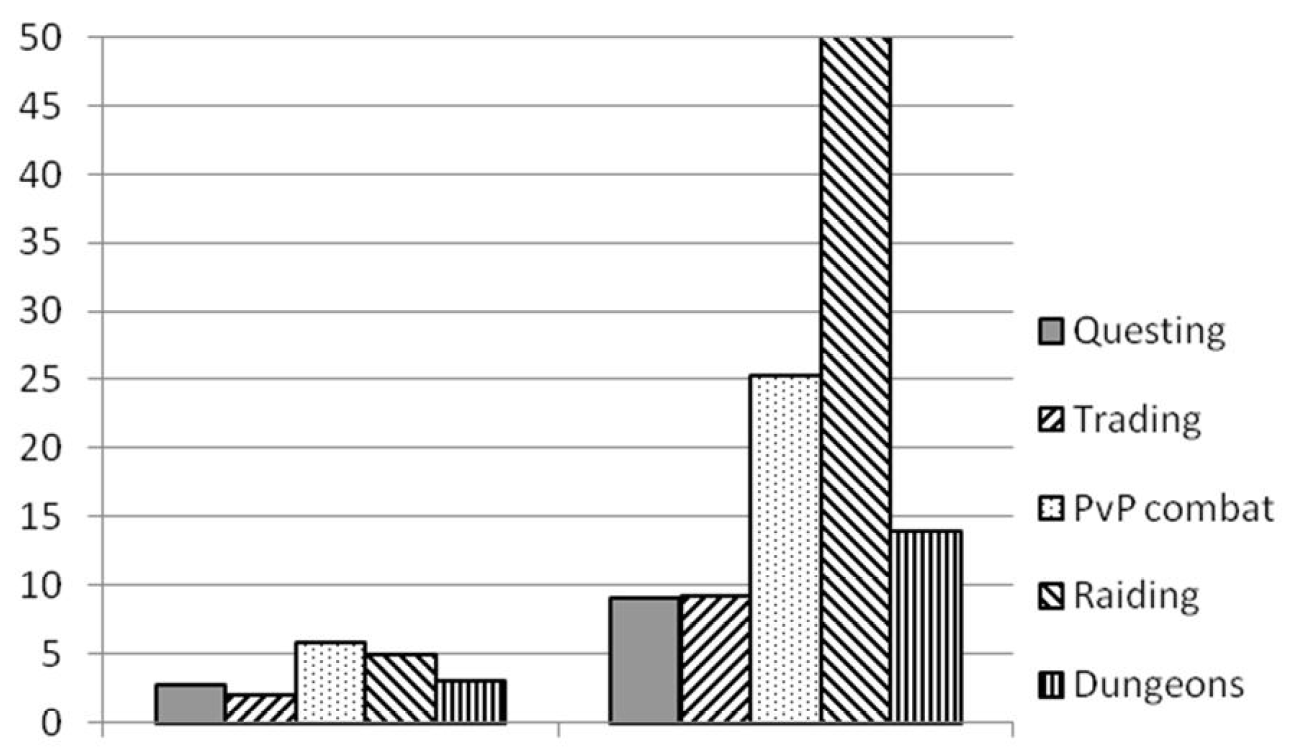
\includegraphics[width=\textwidth]{bande_passante_par_activite.png}\\
		\quad{}Entrante\qquad\qquad\quad{}Sortante\qquad\qquad\quad
	\end{subfigure}
	\\[0.2cm]
	\caption{Bande passante moyenne utilisée dans World of Warcraft en fonction de l'activité~\cite{mmorpg_network_performance_session_patterns_and_latency_requirements_analysis}}
	\label{fig:bande_passante_par_activite}
\end{figure}

\subsubsection{Réseau}
La modélisation du réseau est une partie fondamentale de notre simulateur. Il faut donc pouvoir précisément simuler les interactions réseau que produisent les joueurs. Des études ont été menées sur les déplacements des joueurs de MMORPG en fonction de leur activité pour simuler le réseau utilisé~\cite{mmorpg_network_performance_session_patterns_and_latency_requirements_analysis}~\cite{mmorpg_player_behavior_model}. Les activités d'un joueur de MMORPG peut être classé en différentes catégories : \'Echange (Trading), Quêtes (Questing), Combat Joueur contre Joueur (PvP Combat), Dongeons et Raid. Ces occupations entraînent des activités au niveau du réseau, ainsi que des déplacements, différents selon les joueurs dans le monde virtuel (voir \textsc{Figure}~\ref{fig:bande_passante_par_activite}).\\

Il faut remarquer que la proportion de joueurs dans ces catégories évolue également au cours de la journée. En effet, les raids correspondent à des groupes pré-organisés de joueurs se connectant tous au même moment pour affronter une série d'obstacles. Il est donc naturel que la quantité de joueurs en raid connaisse un pic au même moment que le pic de joueurs. De la même manière, la durée et la probabilité de transition entre ces activités varient au cours du temps et selon l'activité. 
